\chapter{Describing Probabilistic Models}


ToPS uses its own language to describe models and configurations. This is a simple language that will help users without previous knowledge in programming to define the parameters of the model and to do sequence analysis experiments.  

To use a model, you will need to write a configuration file.  The first element of any model configuration file is   a mandatory parameter called "model\_name" that  specify which model you will use. Currently, available "model\_name"  values are:

\begin{itemize}
\item \texttt{DiscreteIIDModel} 
\item \texttt{VariableLengthMarkovChain} 
\item \texttt{HiddenMarkovModel}
\item \texttt{InhomogeneousMarkovChain}
\item \texttt{PairHiddenMarkovModel}
\item \texttt{ProfileHiddenMarkovModel} 
\item \texttt{GeneralizedHiddenMarkovModel}
\end{itemize}

After specifying the model you need to define which is the "alphabet" that will be used, that is, you have to enumerate the input symbols. These can be either single characters, or small words. we show below a few examples
\begin{verbatim}
alphabet={"A","C","G","T"}
alphabet={"Heads", "Tails"}
alphabet={"ATG", "GTT"}
\end{verbatim}
When "alphabet" is not present, ToPS assumes the input symbols are non-negative integer numbers.

After you have specified the model name and the alphabet, you need to specify the rest of the model.
In this chapter we describe how the user can define the specific parameters of each model using simple examples. Finally, we show the formal specification of the language in the Extended Backus-Naur Form (EBNF). 


% ----------------------------------------------------------------- %
\section{Discreet Independent Identically Distributed Model}

We specify a discrete i.i.d. model using a vector of probabilities values. The file \textit{fdd.txt} describes a distribution with two symbols: symbol $Sun$ with probability $0.2$, and symbol $Rain$ with probability $0.8$.

\begin{Verbatim}[frame=single,label=fdd.txt]
model_name = "DiscreteIIDModel"
alphabet = ("Sun", "Rain")
probabilities = (0.2, 0.8)
\end{Verbatim}


As we mentioned above, when the "alphabet" ToPS assumes we are describing the distribution over non-negative integer numbers. For example, the 
file described below is specifying that the probability of $0$ is $0.2$, the probability of $1$ is $0.1$, the probability of $2$ is $0.3$ and the probability of $3$ is $0.4$.

\begin{Verbatim}[frame=single]
model_name = "DiscreteIIDModel"
probabilities = (0.2, 0.1, 0.3, 0.4)
\end{Verbatim}




% ----------------------------------------------------------------- %
\section{Variable Length Markov Chain}

VLMCs are described by specifying  the distribution associated with each context. The  \textit{vlmc.txt} file shows an example. We use the \texttt{probabilities} parameter to specify the conditional probabilities, for example, line 9 specifies that the probability of $X_n = 0$ given that $X_{n-1} = 1$ and $X_{n-2} = 2$ is $0.7$.

\vspace{1em}
\begin{minipage}{\textwidth}
\begin{Verbatim}[frame=single,label={vlmc.txt},numbers=left]
model_name = "VariableLengthMarkovChain"
alphabet = ("0", "1")
probabilities = (
  "0" | "": 0.5; 
  "1" | "": 0.5;
  "0" | "1": 0.5;
  "1" | "1": 0.5;
  "0" | "0": 0.1;
  "1" | "0": 0.9;
  "0" | "1 0": 0.7;#P(X_n=0|X_{n-1}=1,X_{n-2}=0)=0.7
  "1" | "1 0": 0.3; 
  "0" | "1 1": 0.4;
  "1" | "1 1": 0.6)
\end{Verbatim}
\end{minipage}



% ----------------------------------------------------------------- %
\section{Hidden Markov Model}

A simple example where HMM can be used is in the dishonest casino problem. A dishonest casino has two different dice, one is loaded and the other is fair. The casino can change the die without the player knowing, and the challenge is to predict when the casino has changed the dice.  Figure~\ref{fig:hmm-casino} shows the HMM for this problem.  This model has two states (Fair, and Loaded). When the model is in Loaded state there is a greater probability to observe the number one than the other numbers,  and when the model is in Fair state the numbers are uniformly distributed. All the state names are arbitrary and can be freely chosen by the user. A specification of an HMM needs to determine the observation symbols, the states, the various emission probabilities for each state and the transition probabilities between pairs of states.The file below shows an example of HMM described using ToPS:


\begin{Verbatim}[frame=single,label="hmm.txt"]
# Dishonest Casino Problem
model_name="HiddenMarkovModel"
state_names= ("Fair", "Loaded" )
observation_symbols= ("1", "2", "3", "4", "5", "6" )
# transition probabilities
transitions = ("Loaded"    | "Fair": 0.1;
               "Fair"      | "Fair": 0.9;
               "Fair"      | "Loaded": 0.1;
               "Loaded"    | "Loaded": 0.9 )
# emission probabilities
emission_probabilities = ("1" | "Fair" : 0.166666666666; 
                          "2" | "Fair" : 0.166666666666;  
                          "3" | "Fair" : 0.166666666666; 
                          "4" | "Fair" : 0.166666666666; 
                          "5" | "Fair" : 0.166666666666; 
                          "6" | "Fair" : 0.166666666666; 
                          "1" | "Loaded" : 0.5;            
                          "2" | "Loaded" : 0.1;            
                          "3" | "Loaded" : 0.1;            
                          "4" | "Loaded" : 0.1;            
                          "5" | "Loaded" : 0.1;            
                          "6" | "Loaded" : 0.1)            
initial_probabilities= ("Fair": 0.5; "Loaded": 0.5)

\end{Verbatim}

\begin{figure}[!h]
  \centering
  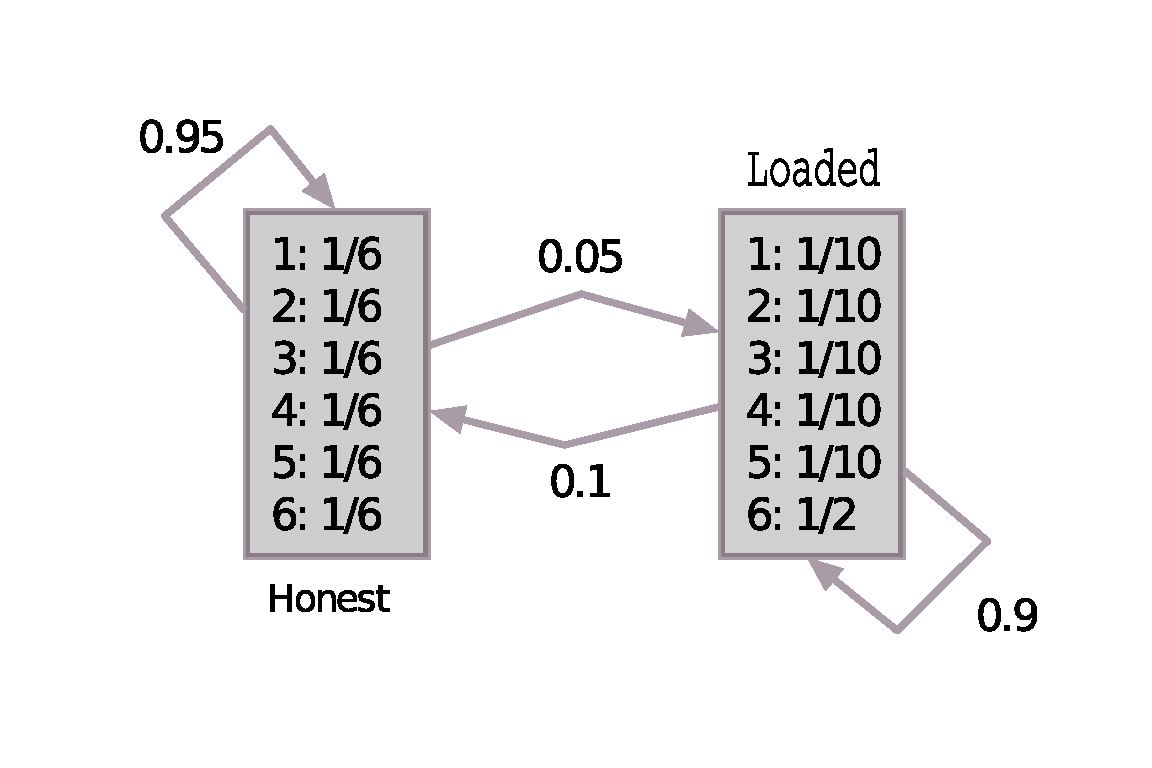
\includegraphics[scale=0.5]{fig_cassino} 
  \caption{Dishonest Casino Problem}
  \label{fig:hmm-casino}
\end{figure}

% ----------------------------------------------------------------- %
\section{Inhomogeneous Markov Model}

To create an inhomogeneous Markov model, we have to specify the conditional probabilities for each position of the sequence. The file \textit{ihm.txt} has  an example of how we can specify this model. There we have three distributions of the symbols "A", "C", "G", "T": p1, p2 and p3.  These names are arbitrary and can be chosen by the user.

\vspace{1em}
\begin{minipage}{\textwidth}
\begin{Verbatim}[frame=single,  label={ihm.txt}]
model_name = "InhomogeneousMarkovChain"
alphabet = ("A", "C", "G", "T")
p1 = ("A" | "" : 0.97;
      "C" | "" : 0.01;
      "G" | "" : 0.01 ;
      "G" | "" : 0.01)
p2 = ("A" | "" : 0.01;
      "C" | "" : 0.97;
      "G" | "" : 0.01 ;
      "G" | "" : 0.01)
p3 = ("A" | "" : 0.01;
      "C" | "" : 0.01;
      "G" | "" : 0.97 ;
      "G" | "" : 0.01)
position_specific_distribution = ("p1","p2","p3")
phased =0
\end{Verbatim}
\end{minipage}
\vspace{1em}

The \textit{position\_specific\_distribution} argument  uses the parameters p1, p2, and p3 to specify respectively the distributions for the positions 1, 2, and 3 of the sequence. 

In this example the \textit{phased} parameter, with value equals to zero, is specifying that the model is describing fixed-length sequences.  A model that represents fixed-length sequences is useful when we want to model biological signal. Weight Array Model~\cite{Zhang1993} is an example of this type of Inhomogeneous Markov Chain.

If the \textit{phased} is equal to one, then the sequences are generated  using  periodically the distributions p1, p2, and p3. In other words, p1 is used in positions 1, 4, 7 and so on; p2 is used in positions 2, 5, 8 and so on; p3 is used in positions 3, 6, 9 and so on. This behaviour is useful to model coding regions of the gene. Three-periodic Markov chain~\cite{Borodovsky1993} is an example of a inhomogeneous Markov Chain with phased  equals to 1 and three position specific distributions.


% ----------------------------------------------------------------- %
\section{Pair Hidden Markov Model}\label{pairHMMModelDesc}

A very common problem when analyzing biological sequences is that of aligning a pair of sequences. This task can be accomplished with he use of decodable models, although in this case these models must be able to handle a pair of sequences simultaneously. Here we describe who to use ToPS to specify pair hidden Markov models (pair-HMM). This specify pair-HMM has a Match state (M),  two insertion states (I1, I2), two deletion states (D1, D2) an initial state (B), and a final state (E). All the state names are arbitrary and can be freely chosen by the user.Similar to HMMs, a pair-HMM specification need to determine the observation symbols, the states, the various emission probabilities for each state and the transition probabilities between pairs of states.

\vspace{1em}
\begin{Verbatim}[frame=single,  label={ihm.txt}]
model_name="PairHiddenMarkovModel"
state_names = ("M", "I1", "D1", "I2", "D2", "B", "E")
observation_symbols = ("A","C","G","T")
transitions = ("M" | "B" :0.9615409374;
		"I1" | "B" : 4.537999985e-07;
		"D1" | "B" : 4.537999985e-07;
		"I2" | "B" : 0.01922916807;
		"D2" | "B" : 0.01922916807;
		"I1" | "M" : 0.01075110921;
		"D1" | "M" : 0.01075110921;
		"I2" | "M" : 0.008213998383;
		"D2" | "M" : 0.008213998383;
		"M" | "M" : 0.9619031182;
		"I1" | "I1" : 0.3209627509;
		"D1" | "D1" : 0.3209627509;
		"I2" | "I2" : 0.3297395944;
		"D2" | "D2" : 0.3297395944;
		"M" | "I1" : 0.6788705825;
		"M" | "D1" : 0.6788705825;
		"M" | "I2" : 0.670093739;
		"M" | "D2" : 0.670093739;
		"E" | "M" : 0.000166667;
		"E" | "I1" : 0.000166667;
		"E" | "D1" : 0.000166667;
		"E" | "I2" : 0.000166667;
		"E" | "D2" : 0.000166667;)
emission_probabilities = ("AA" | "M" : 0.1487240046;
			"AT" | "M" : 0.0238473993;
			"AC" | "M" : 0.0184142999;
			"AG" | "M" : 0.0361397006;
			"TA" | "M" : 0.0238473993;
			"TT" | "M" : 0.1557479948;
			"TC" | "M" : 0.0389291011;
			"TG" | "M" : 0.0244289003;
			"CA" | "M" : 0.0184142999;
			"CT" | "M" : 0.0389291011;
			"CC" | "M" : 0.1583919972;
			"CG" | "M" : 0.0275536999;
			"GA" | "M" : 0.0361397006;
			"GT" | "M" : 0.0244289003;
			"GC" | "M" : 0.0275536999;
			"GG" | "M" : 0.1979320049;
			"A-" | "I1" : 0.2270790040;
			"T-" | "I1" : 0.2464679927;
			"C-" | "I1" : 0.2422080040;
			"G-" | "I1" : 0.2839320004;
			"-A" | "D1" : 0.2270790040;
			"-T" | "D1" : 0.2464679927;
			"-C" | "D1" : 0.2422080040;
			"-G" | "D1" : 0.2839320004;
			"A-" | "I2" : 0.2270790040;
			"T-" | "I2" : 0.2464679927;
			"C-" | "I2" : 0.2422080040;
			"G-" | "I2" : 0.2839320004;
			"-A" | "D2" : 0.2270790040;
			"-T" | "D2" : 0.2464679927;
			"-C" | "D2" : 0.2422080040;
			"-G" | "D2" : 0.2839320004;)
number_of_emissions = ("M" : "1,1";
			"I1" : "1,0";	
			"D1" : "0,1";
			"I2" : "1,0";	
			"D2" : "0,1";	
			"B" : "0,0";
			"E" : "0,0")
\end{Verbatim}


% ----------------------------------------------------------------- %
\section{Profile Hidden Markov Model}


Biologial sequences usually come in families and a very common problem when analyzing this sequences is identify the relationship of an individual sequence to a sequence family. Profile HMMs are variations of HMMs with three types of states: Match states, Insertion States and Deletion States. Deletion States have no emission probabilities. Profile-HMMs were  designed to classify a family os sequences based on  a multiple sequence alignment. Our example below (file  \textit{profilehmm.txt})  has five match states $ M0, M1, M2, M3, M4 $ ($M0$ and $M4$ are modeled as the begin and end states respectively), four insert states $ I0, I1, I2, I3 $ and three delete states $D1, D2, D3$.
 \pagebreak

\vspace{1em}
\begin{Verbatim}[frame=single,  label={profilehmm.txt}]
model_name = "ProfileHiddenMarkovModel"
state_names = ("M0","M1","M2","M3","M4","I0","I1","I2","I3",
		"D1","D2","D3")
observation_symbols = ("A","C","G","T")
transitions = ("M1" | "M0": 0.625;
		"I0" | "M0": 0.125;
		"D1" | "M0": 0.25;
		"M2" | "M1": 0.714286;
		"I1" | "M1": 0.142857;
		"D2" | "M1": 0.142857;
		"M3" | "M2": 0.428571;
		"I2" | "M2": 0.428571;
		"D3" | "M2": 0.142857;
		"M4" | "M3": 0.833333;
		"I3" | "M3": 0.166667;
		"M4" | "M4": 1;
		"M1" | "I0": 0.333333;
		"I0" | "I0": 0.333333;
		"D1" | "I0": 0.333333;
		"M2" | "I1": 0.333333;
		"I1" | "I1": 0.333333;
		"D2" | "I1": 0.333333;
		"M3" | "I2": 0.272727;
		"I2" | "I2": 0.545455;
		"D3" | "I2": 0.181818;
		"M4" | "I3": 0.5;
		"I3" | "I3": 0.5;
		"M2" | "D1": 0.25;
		"I1" | "D1": 0.25;
		"D2" | "D1": 0.5;
		"M3" | "D2": 0.25;
		"I2" | "D2": 0.5;
		"D3" | "D2": 0.25;
		"M4" | "D3": 0.666667;
		"I3" | "D3": 0.333333)
emission_probabilities = ("A" | "M1": 0.5;
		"C" | "M1": 0.125;
		"G" | "M1": 0.25;
		"T" | "M1": 0.125;
		"A" | "M2": 0.25;
		"C" | "M2": 0.125;
		"G" | "M2": 0.5;
		"T" | "M2": 0.125;
		"A" | "M3": 0.125;
		"C" | "M3": 0.625;
		"G" | "M3": 0.125;
		"T" | "M3": 0.125;
		"A" | "I0": 0.25;
		"C" | "I0": 0.25;
		"G" | "I0": 0.25;
		"T" | "I0": 0.25;
		"A" | "I1": 0.25;
		"C" | "I1": 0.25;
		"G" | "I1": 0.25;
		"T" | "I1": 0.25;
		"A" | "I2": 0.5;
		"C" | "I2": 0.25;
		"G" | "I2": 0.166667;
		"T" | "I2": 0.0833333;
		"A" | "I3": 0.25;
		"C" | "I3": 0.25;
		"G" | "I3": 0.25;
		"T" | "I3": 0.25)
initial_probabilities = ("M0": 1)

\end{Verbatim}

Profile HMMs can also be automatically inferred from multiple sequence alignments (see Training). 
% ----------------------------------------------------------------- %
\section{Generalized Hidden Markov Model}

GHMMs are useful in Bioinformatics to represent the structure of genes. With GHHMs each state can have an arbitrary probabilistic model as a sub-model. Also, we can specify the durations of states either by a self transition with a given probability value or as a distribution over integer numbers.  As an illustrative  example we will use a simplified  model for a bacterial gene. In bacteria, genes are regions of the genome with a different composition, specific start and stop signals, and  noncoding regions separating different genes.  Figure~\ref{fig:ghmm} illustrates this gene model. The model has four states:   $NonCoding$ state, representing the intergenic regions, with geometric duration distribution (represented by a self transition in the figure); $Start$ and $Stop$ states , representing  the signals at the boundaries of a gene, with a fixed duration distribution (with value 3); $Coding$,  representing the coding region of a gene, with  an i.i.d.  duration distribution (ideally this would be associated with the size distribution of bacterial genes).  Box  \textit{ghmm.txt} shows the description of this GHMM.

\begin{figure}[htpb]
  \centering
  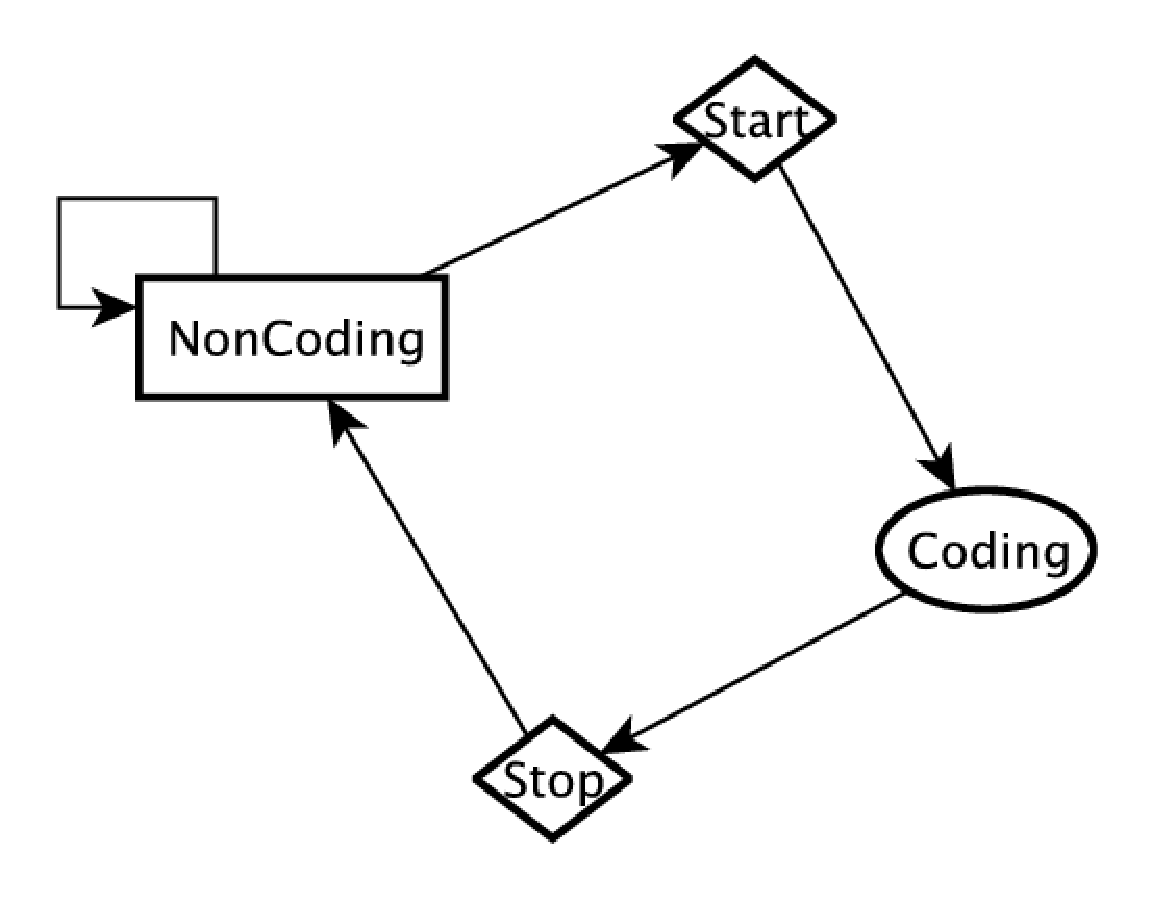
\includegraphics[width=0.35\textwidth]{ghmm}
  \caption{GHMM that represents protein-coding genes in bacteria.}
  \label{fig:ghmm}
\end{figure}


The parameters \textit{state\_names}, \textit{observation\_symbols}, \textit{initial\_proba\-bilities}, and \textit{transi\-tions} are configured in the same way as in the case of  the HMM model, described above.

We have to specify the models that the GHMM will use, either by naming a file that contains its description or by inlining its description in the GHMM specification file. In our example, the GHMM uses five submodels: (i) \textit{noncoding\_model} (a \textit{DiscreteIIDModel} inlined in the GHMM specification); (ii) \textit{coding\_model} ( in file ``coding.txt'') ; (iii) \textit{start\_model} ( in file ``start.txt''); (iv) \textit{stop\_model} (in file ``stop.txt''); (v) \textit{coding\_duration\_model} (in file ``coding\_duration.txt'').

After specifying the models, we have to describe the configuration of each state. ToPS assumes that the GHMM has two classes of states: (i) Fixed-length  states, that  emit fixed length words, and  (ii) variable-length states, that emit words with lengths given by a probability distribution. There are two types of variable-length states:  states with geometric distributed duration and states with non-geometric distributed duration. When specifying any state, the user have to specify the observation model using the parameter \textit{observation}. States with geometric duration distribution are specified with a self transition, states with  fixed-length dueation the user should use the parameter \textit{sequence\_length}, and other states should use the  parameter \textit{duration}.

In the file \textit{ghmm.txt}, we have two fixed-length states (\textit{Start}, and \textit{Stop}) and two variable-length states (\textit{NonCoding}, and \textit{Coding}):
\begin{itemize}
  \item \textit{Start} state, with \textit{start\_model} as the observation model.
\item\textit{Stop} state, with \textit{stop\_model} as  the observation model. 
\item \textit{NonCoding} state, with   \textit{noncoding\_model} as the observation model, and durations  given by a geometric distribution in which the probability of staying in the same state is $0.999$. 
\item \textit{Coding} state,  with \textit{coding\_model} as the observation model, and durations  given by the \textit{coding\_duration\_model}.
\end{itemize}


\begin{Verbatim}[frame=single,  label={ghmm.txt}]
model_name = "GeneralizedHiddenMarkovModel"
state_names =
  ("NonCoding",
   "Start",
   "Coding",
   "Stop")
observation_symbols =
  ("A", "C", "G", "T")
initial_probabilities =
  ("NonCoding": 1.0)
transitions =
  ("NonCoding"  | "NonCoding": 0.999;
        "Start" | "NonCoding": 0.001;
       "Coding" | "Start": 1.0;
         "Stop" | "Coding": 1.0;
   "NonCoding"  | "Stop": 1.0)
noncoding_model =
  [ model_name = "DiscreteIIDModel"
    alphabet = ("A", "C", "G", "T")
    probabilities=(0.25, 0.25, 0.25, 0.25)]
coding_model = "coding.txt"
start_model = "start.txt"
stop_model = "stop.txt"
coding_duration_model="coding_duration.txt"
NonCoding =
  [ observation = noncoding_model ]
Start =
  [ observation =start_model
    sequence_length = 15 ]
Stop =
  [ observation = stop_model
    sequence_length = 15 ]
Coding =
  [ observation = coding_model
    duration = coding_duration_model ]
\end{Verbatim}

% ----------------------------------------------------------------- %

\section{Language Description (EBNF)}

The configuration file of ToPS contains a list of defined properties. Each property is associated with a value that can be a string, integer, float number, a list of string, a list of numbers, conditional probabilities, or a list of other properties.  Below, we describe the formal language description of ToPS in the Extended Backus-Naur Form (EBNF):

\begin{lstlisting}[frame=trbl]
model                          : properties
                               ;
                               
properties                     : property
                               | properties property
                               ;
                               
property                       : IDENTIFIER '=' value
                               ;
                               
value                          : STRING
                               | INTEGER_NUMBER
                               | FLOAT_POINT_NUMBER
                               | list
                               | probability_map
                               | conditional_probability_map
                               | sub_model
                               | IDENTIFIER
                               ;
                               
list                           : '(' list_elements ')'
                               ;
                               
list_elements                  : list_element
                               | list_elements ',' list_element
                               ;
                               
list_element                   : STRING
                               | INTEGER_NUMBER
                               | FLOAT_POINT_NUMBER
                               ;
                               
probability_map                : '(' probabilities_list ')'
                               ;
                               
probabilities_list             : probabilities
                               | probabilities ';'
                               ;
                               
probabilities                  : probability
                               | probabilities ';' probability
                               ;
                               
probability                    : STRING ':' list_element
                               ;

conditional_probability_map    : '(' conditional_probabilities_list ')'
                               ;

conditional_probabilities_list : conditional_probabilities
                               | conditional_probabilities ';'
                               ;

conditional_probabilities      : conditional_probability
                               | conditional_probabilities ';' conditional_probability
                               ;

conditional_probability        : condition ':' probability_number
                               ;

condition                      : STRING '|' STRING
                               ;

probability_number             : INTEGER_NUMBER
                               | FLOAT_POINT_NUMBER
                               ;

sub_model                      : '[' properties ']'
                               ;
\end{lstlisting}

And the tokens are defined by the following regular expressions:

\begin{lstlisting}[frame=trbl]
IDENTIFIER         : [a-zA-Z_][a-zA-Z0-9_]*
STRING             : L?\"(\\.|[^\\"])*\"
COMMENTS           : "#"[^\r\n]*
FLOAT_POINT_NUMBER : [0-9]+\.[0-9]+([Ee][+-]?[0-9]+)?
INTEGER_NUMBER     : [0-9]+
\end{lstlisting}


